%%%%%%%%%%%%%%%%%%%%%%%%%%%%%%%%%%%%%%%%%%%%%%%%%%%%%%%%%%%%%%%%%%%%
%% I, the copyright holder of this work, release this work into the
%% public domain. This applies worldwide. In some countries this may
%% not be legally possible; if so: I grant anyone the right to use
%% this work for any purpose, without any conditions, unless such
%% conditions are required by law.
%%%%%%%%%%%%%%%%%%%%%%%%%%%%%%%%%%%%%%%%%%%%%%%%%%%%%%%%%%%%%%%%%%%%

\documentclass{beamer}
\usetheme[university=bs,faculty=standard]{fibeamer}
\usepackage[utf8]{inputenc}
\usepackage[
  main=italian, %% By using `italian`as the main locale
                %% instead of `english`, you can typeset the
                %% presentation in Italian.
  english       %% The additional key allow foreign texts to be
]{babel}        %% typeset as follows:
%%
%%   \begin{otherlanguage}{italian}   ... \end{otherlanguage}
%%
%% These macros specify information about the presentation
\title{Personaggi in Fate/Grand Order} %% that will be typeset on the
%\subtitle{Presentation Subtitle} %% title page.
\author{Lucchi Manuele, Tricella Davide}

%% These additional packages are used within the document:
\usepackage{ragged2e}  % `\justifying` text
\usepackage{booktabs}  % Tables
\usepackage{tabularx}
\usepackage{tikz}      % Diagrams
\usetikzlibrary{calc, shapes, backgrounds}
\usepackage{amsmath, amssymb}
\usepackage{url}       % `\url`s
\usepackage{listings}  % Code listings
\usepackage{graphicx}
\usepackage{varwidth}

\frenchspacing
\begin{document}
\frame[c]{\maketitle}

\begin{darkframes}

  \section{Presentazione}

  \begin{frame}{Introduzione}
    \framesubtitle{Servant}
    \begin{columns}
      \begin{column}{0.5\textwidth}
        \textbf{Dataset} (da \textbf{Atlas Academy})
        \begin{itemize}
          \item DisplayName
          \item Class
          \item Rarity
          \item ATK (e relativi)
          \item HP (e relativi)
          \item Traits
          \item Attribute
          \item Illustrator
        \end{itemize}
      \end{column}
      \begin{column}{0.5\textwidth}
        \begin{figure}
          \centering
          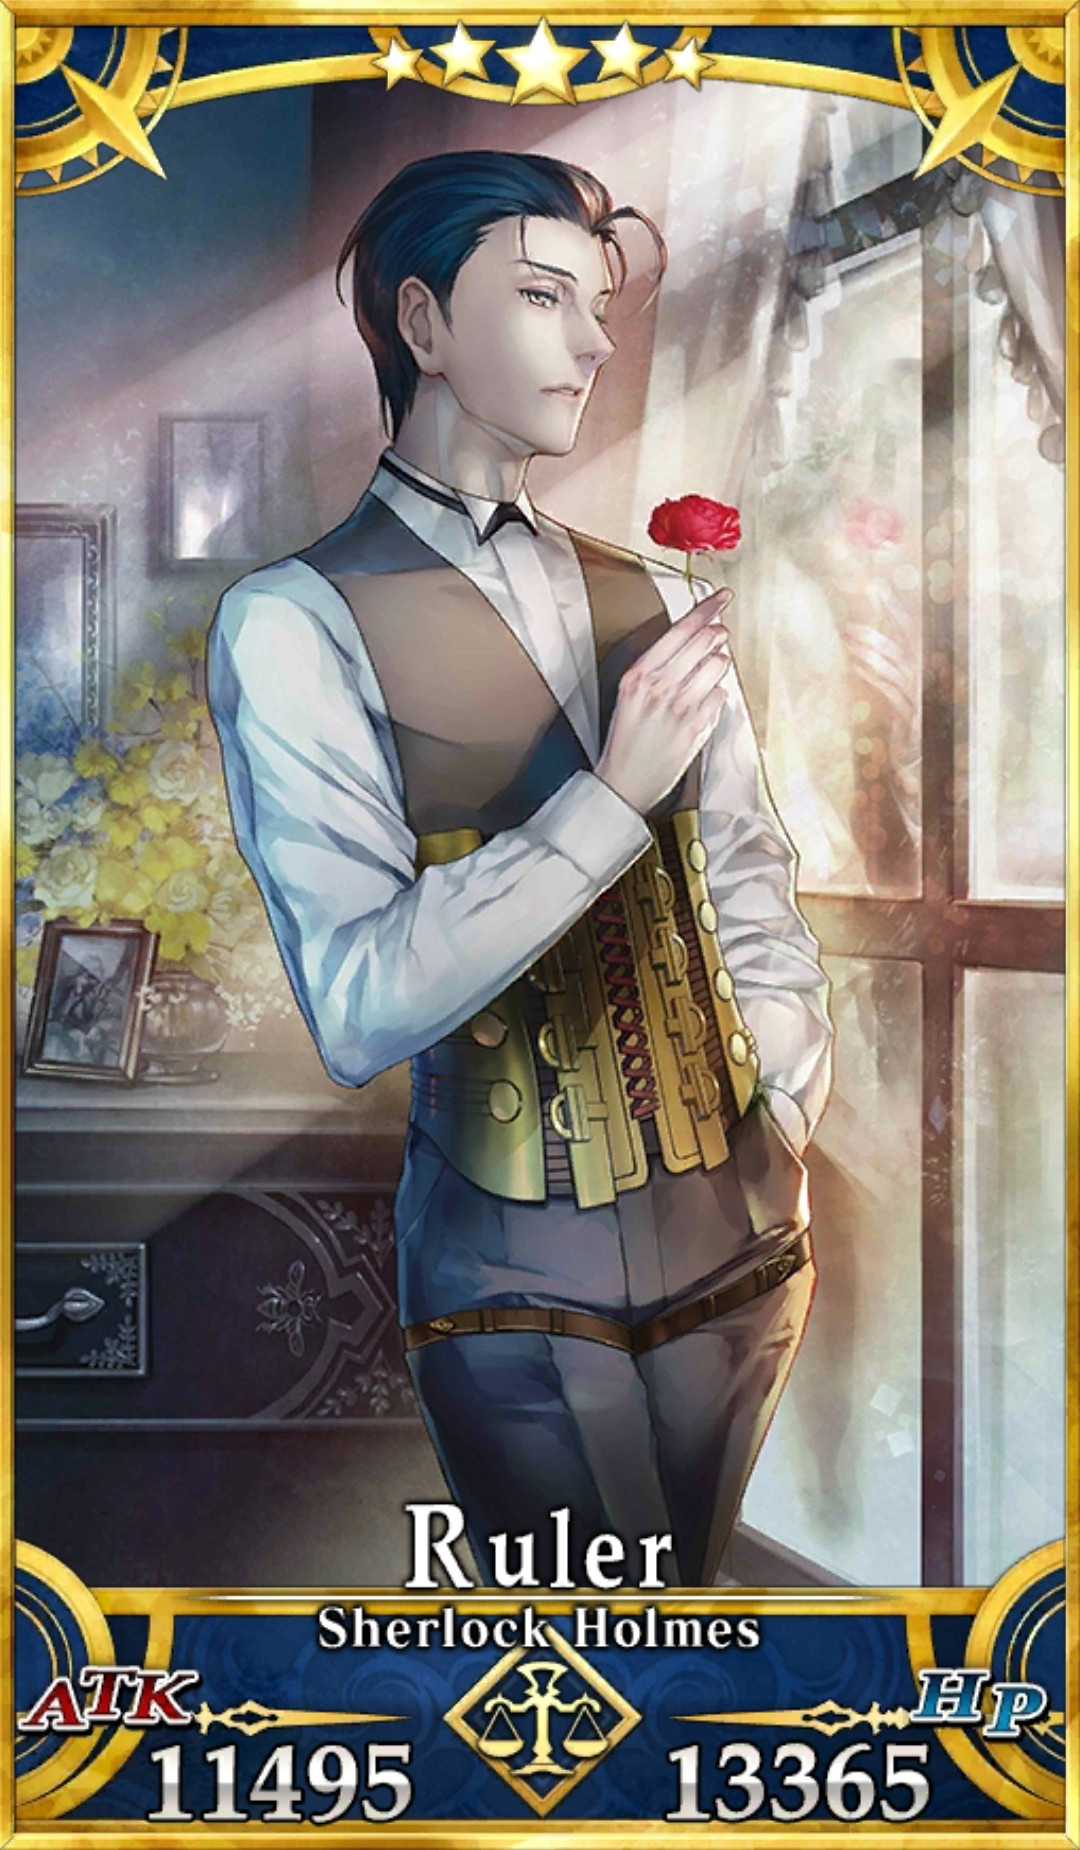
\includegraphics[height=0.65\textheight]{./images/servant.png}
        \end{figure}
      \end{column}
    \end{columns}
  \end{frame}

  \begin{frame}{Classe}
    \begin{columns}
      \begin{column}{0.5\textwidth}
        Classe del servant, identifica le affinità a livello di gameplay e storia
      \end{column}
      \begin{column}{0.5\textwidth}
        \begin{figure}
          \centering
          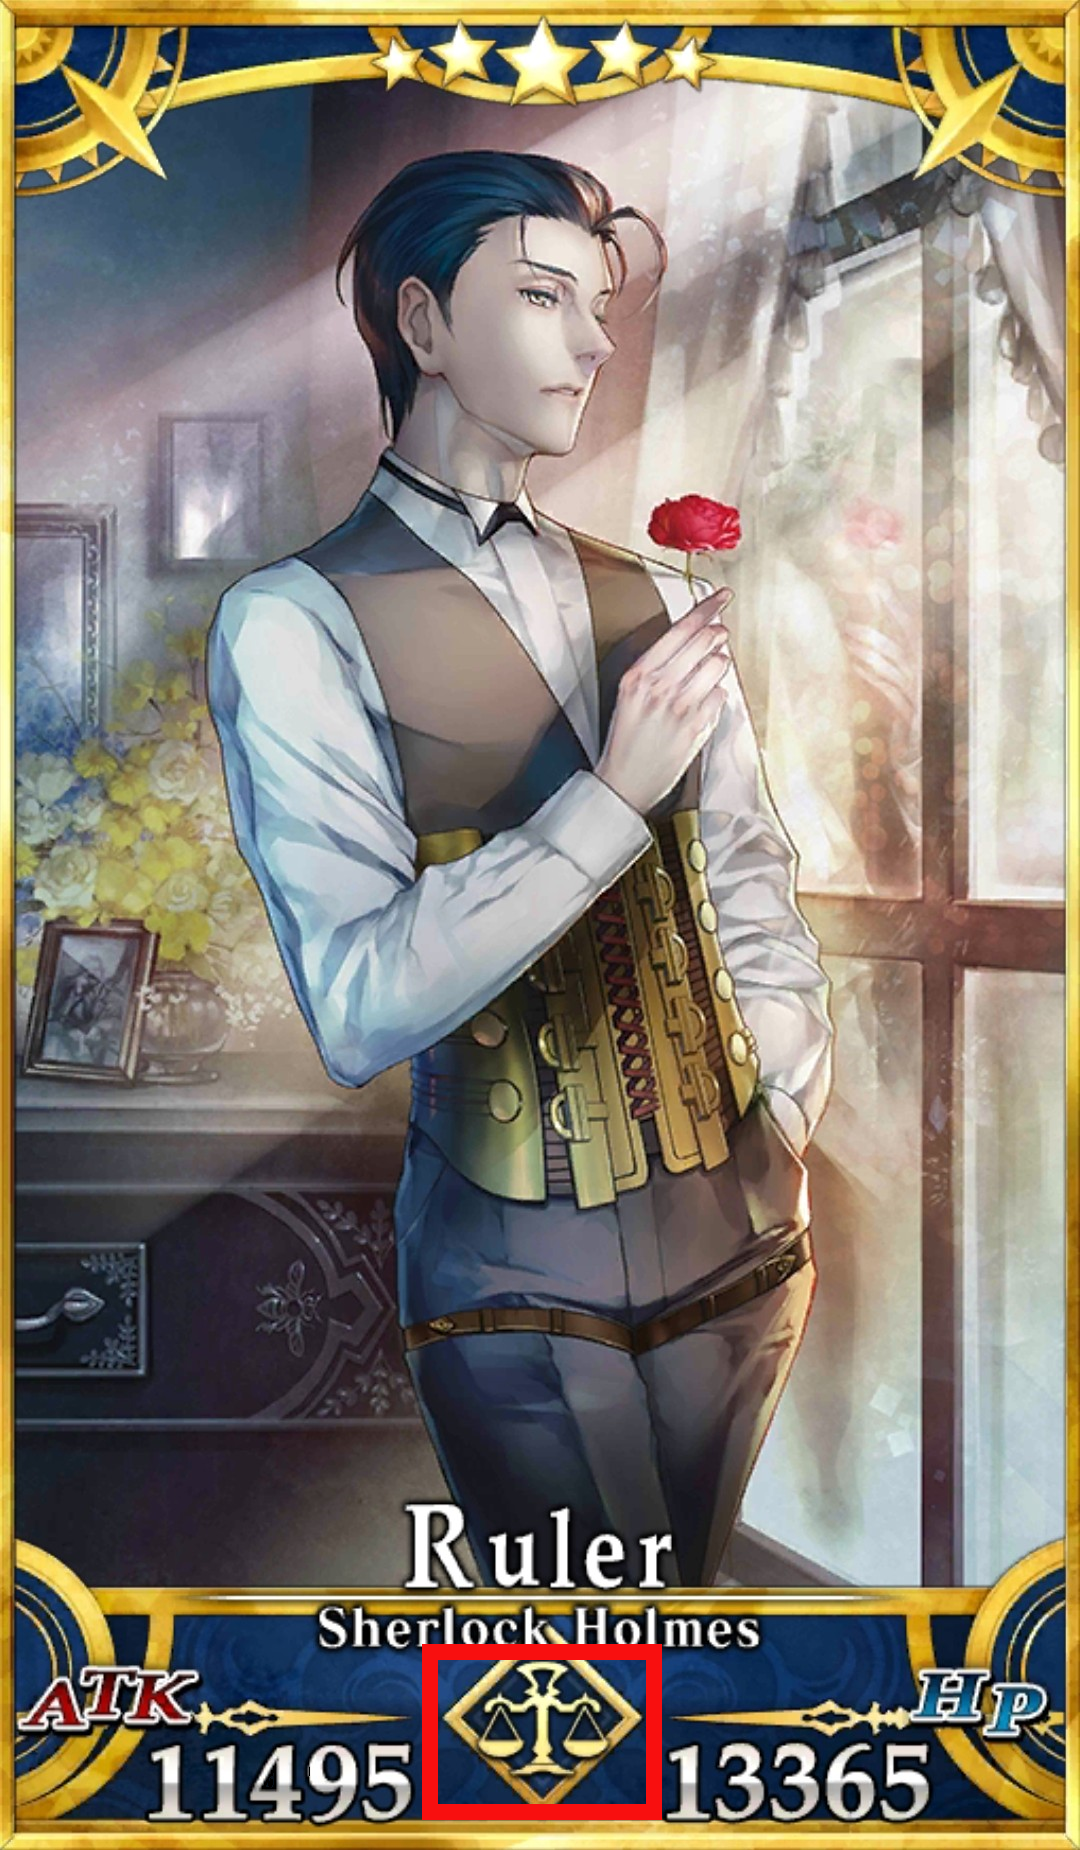
\includegraphics[height=0.65\textheight]{./images/servant_class.png}
        \end{figure}
      \end{column}
    \end{columns}
  \end{frame}

  \begin{frame}{Classi}
    \begin{figure}
      \centering
      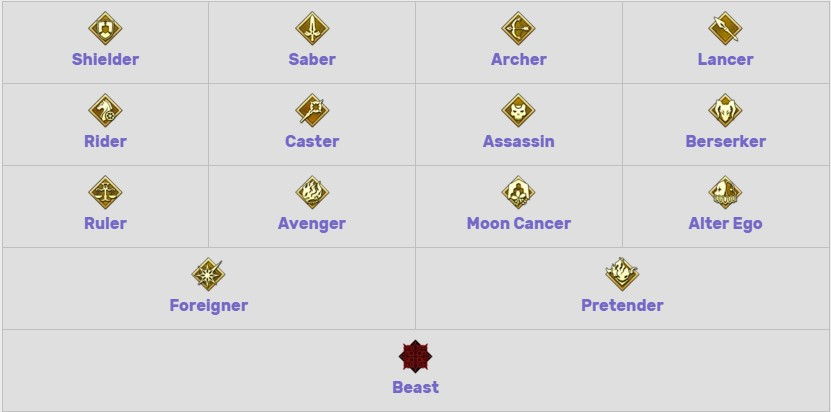
\includegraphics[height=0.55\textheight]{./images/classes.jpg}
    \end{figure}
  \end{frame}

  \begin{frame}{Classi}
    \begin{figure}
      \centering
      
\includegraphics[scale=0.65]{./images/frequency_by_class.png}
    \end{figure}
  \end{frame}

  \begin{frame}{Attributi}
    \begin{columns}
      \begin{column}{0.25\textwidth}
        L'attributo non è visibile nella card del servant
        \begin{itemize}
          \item Earth
          \item Human
          \item Sky
          \item Star
        \end{itemize}
      \end{column}
      \begin{column}{0.75\textwidth}
        \begin{figure}
          \centering
          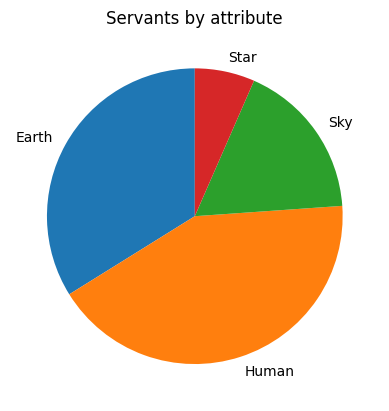
\includegraphics[scale=0.65]{./images/frequency_by_attribute.png}
        \end{figure}
      \end{column}
    \end{columns}
  \end{frame}

  \begin{frame}{Rarità}
    \framesubtitle{Da 0 a 5 stelle}
    \begin{columns}
      \begin{column}{0.5\textwidth}
        Identifica il grado e la difficoltà nell'ottenerlo, influenza determinate statistiche
      \end{column}
      \begin{column}{0.5\textwidth}
        \begin{figure}
          \centering
          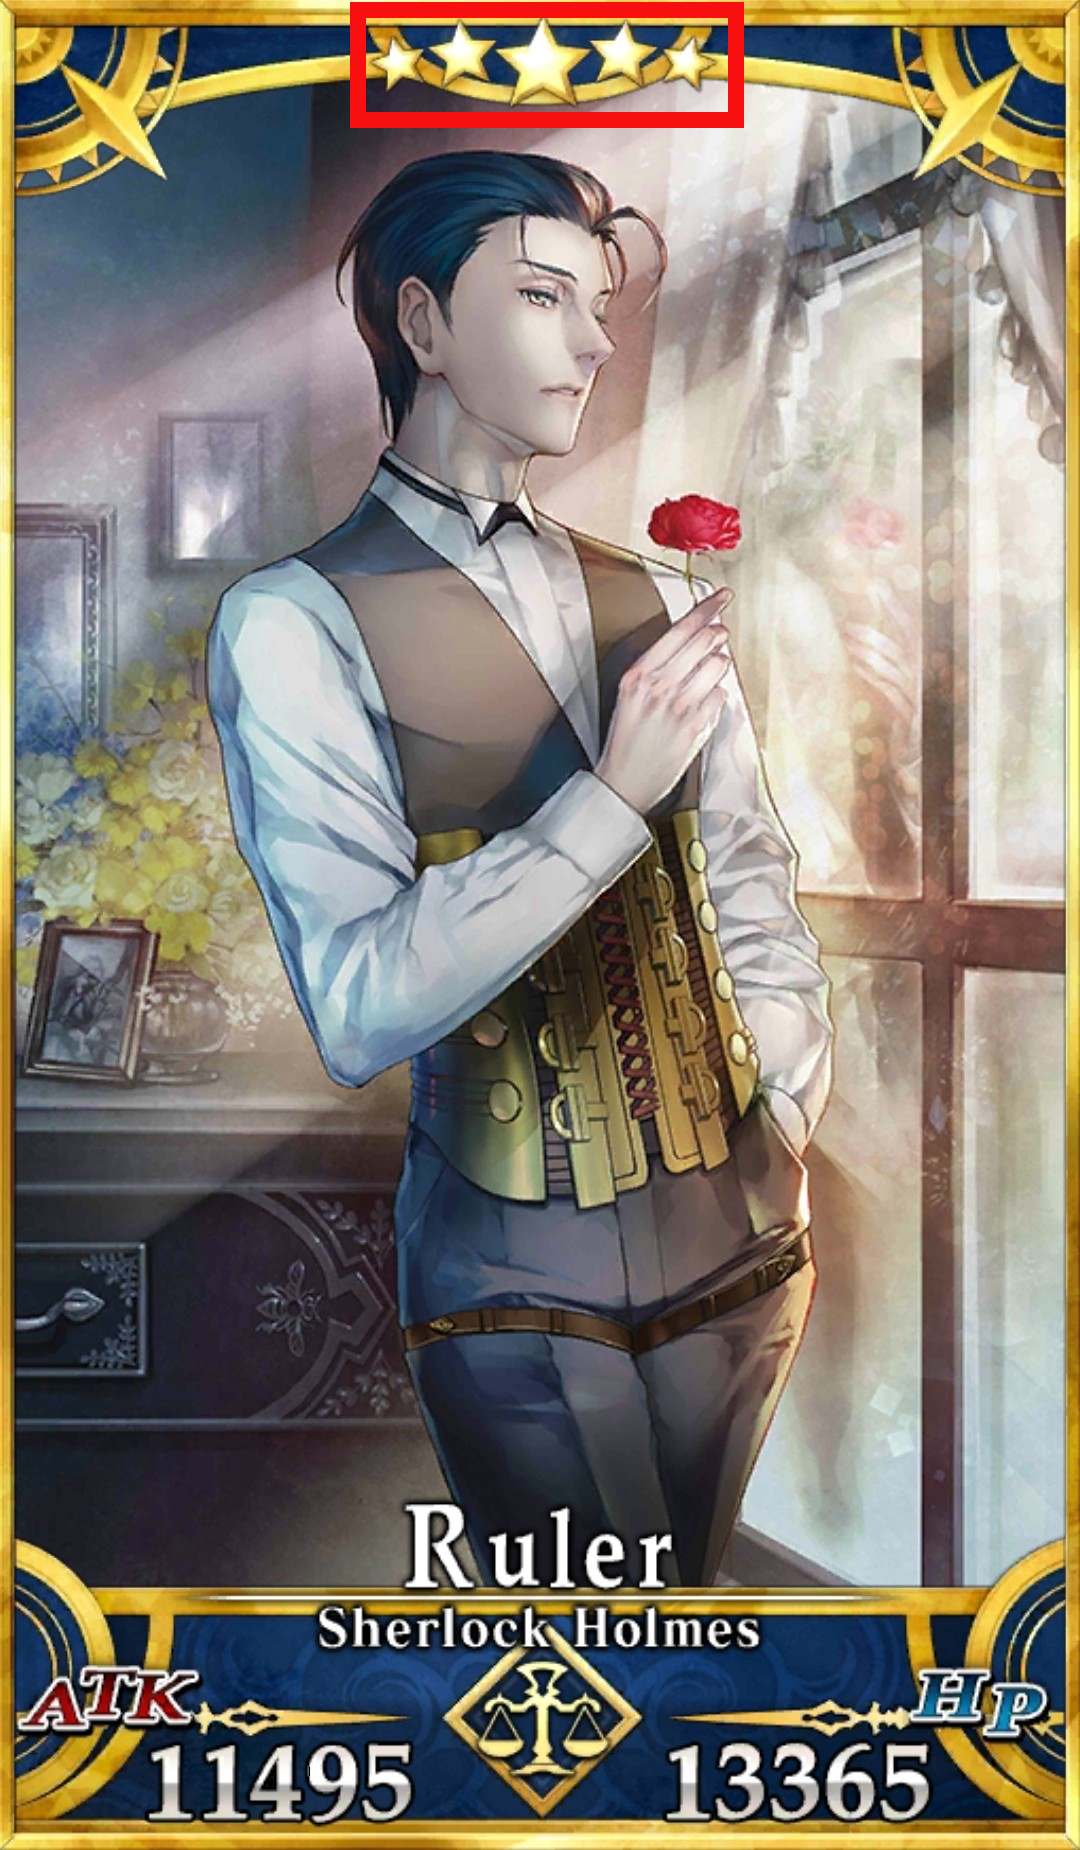
\includegraphics[height=0.65\textheight]{./images/servant_rarita.png}
        \end{figure}
      \end{column}
    \end{columns}
  \end{frame}

  \begin{frame}{Rarità}
    \framesubtitle{Da 0 a 5 stelle}
    \begin{figure}
      \centering
      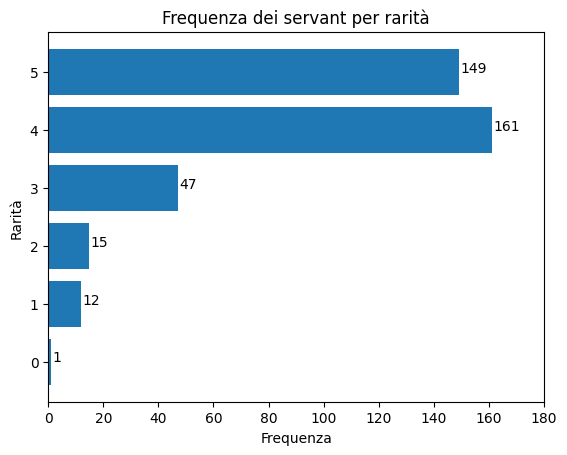
\includegraphics[scale=0.60]{./images/frequency_by_rarity.png}
    \end{figure}
  \end{frame}

  \begin{frame}{Rarità}
    \framesubtitle{Uscite nel tempo}
    \begin{figure}
      \centering
      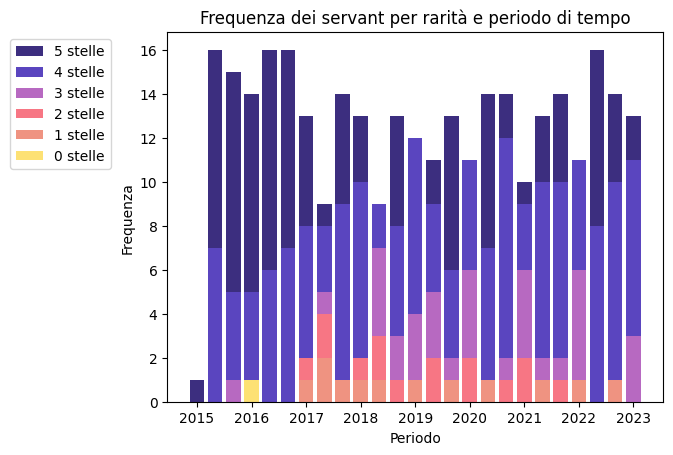
\includegraphics[scale=0.6]{./images/rarity_per_year_bar.png}
    \end{figure}
  \end{frame}

  \begin{frame}{Statistiche}
    \framesubtitle{Statistiche di attacco e punti vita}
    \begin{columns}
      \begin{column}{0.5\textwidth}
        Identificano i danni e il grado di sopravvivenza del servant
      \end{column}
      \begin{column}{0.5\textwidth}
        \begin{figure}
          \centering
          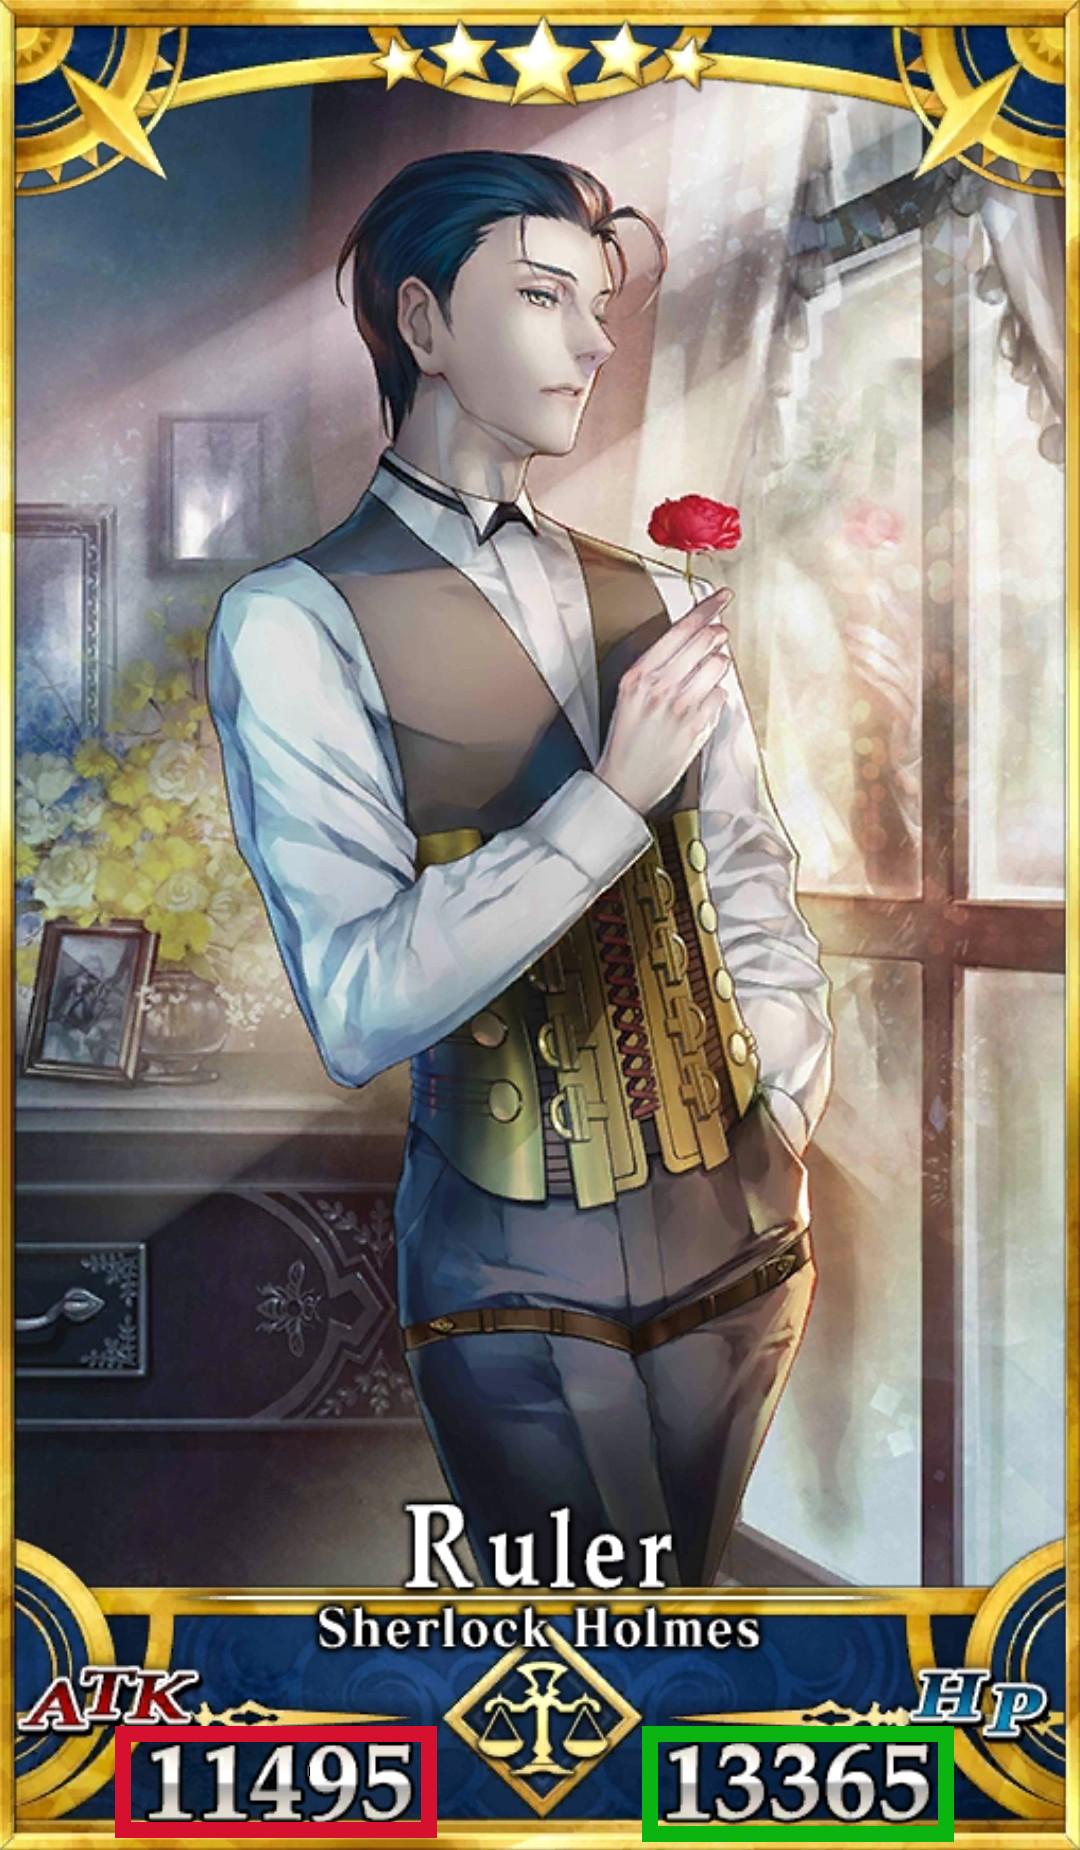
\includegraphics[height=0.65\textheight]{./images/servant_atk_hp.png}
        \end{figure}
      \end{column}
    \end{columns}
  \end{frame}

  \begin{frame}{Statistiche}
    \framesubtitle{Statistiche di attacco}
    \begin{figure}
      \centering
      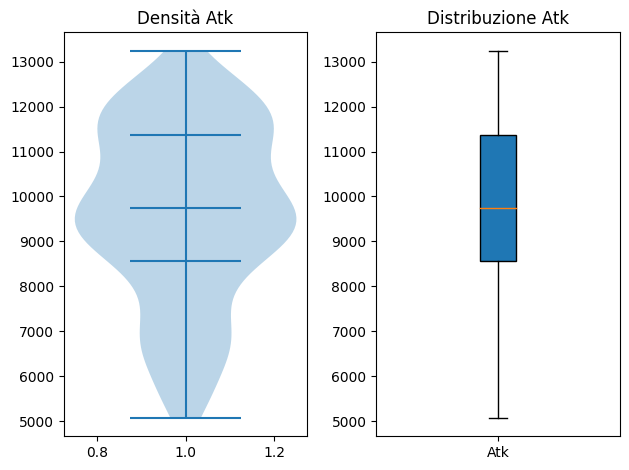
\includegraphics[scale=0.6]{./images/box_atk.png}
    \end{figure}
  \end{frame}

  \begin{frame}{Statistiche}
    \framesubtitle{Statistiche di punti vita}
    \begin{figure}
      \centering
      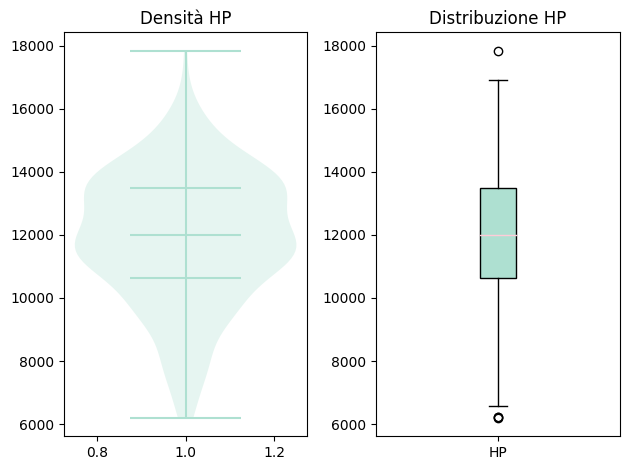
\includegraphics[scale=0.6]{./images/box_hp.png}
    \end{figure}
  \end{frame}

  \begin{frame}{Statistiche}
    \framesubtitle{Statistiche di attacco legate alla rarità}
    \begin{figure}
      \centering
      
\includegraphics[scale=0.6]{./images/class_and_stats_atk.png}
    \end{figure}
  \end{frame}

  \begin{frame}{Statistiche}
    \framesubtitle{Statistiche di punti vita legate alla rarità}
    \begin{figure}
      \centering
      
\includegraphics[scale=0.6]{./images/class_and_stats_hp.png}
    \end{figure}
  \end{frame}

  \begin{frame}{Statistiche}
    \framesubtitle{Crescita delle statistiche all'avanzare del livello}
    \begin{figure}
      \centering
      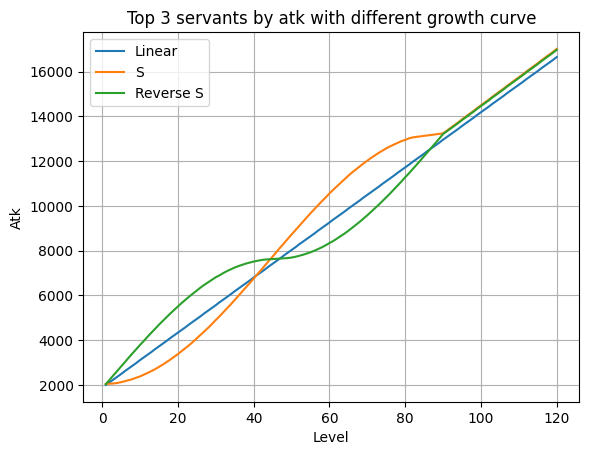
\includegraphics[scale=0.6]{./images/growth.png}
    \end{figure}
  \end{frame}

  \begin{frame}{Statistiche}
    \framesubtitle{Statistiche di classi a confronto}
    \begin{figure}
      \centering
      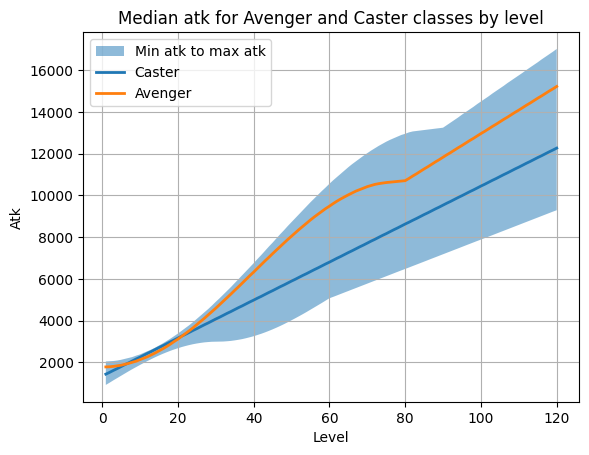
\includegraphics[scale=0.6]{./images/caster_vs_avenger.png}
    \end{figure}
  \end{frame}

  \begin{frame}{Illustratori}
    \begin{figure}
      \centering
      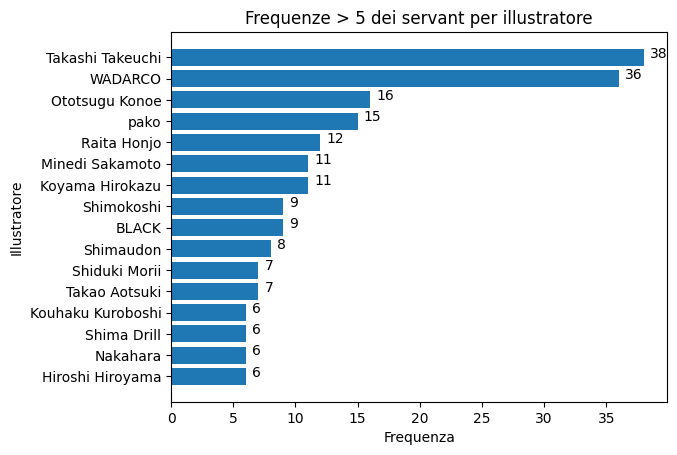
\includegraphics[scale=0.55]{./images/illustrators.png}
    \end{figure}
  \end{frame}

  \begin{frame}{Illustratori}
    \framesubtitle{Illustrazioni e traits}
    \begin{columns}
      \begin{column}{0.50\textwidth}
        \begin{figure}
          \centering
          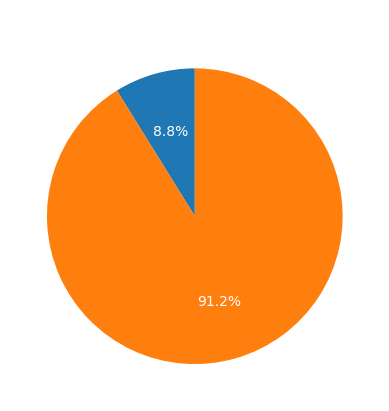
\includegraphics[scale=0.55]{./images/saberface.png}
        \end{figure}
      \end{column}
      \begin{column}{0.50\textwidth}
        \begin{figure}
          \centering
          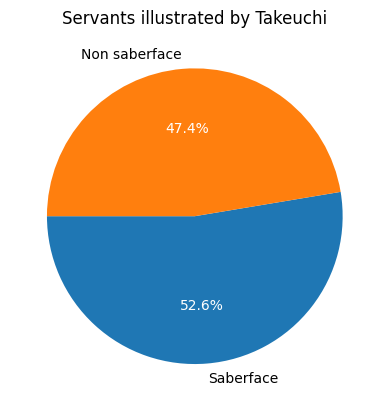
\includegraphics[scale=0.55]{./images/saberface_take.png}
        \end{figure}
      \end{column}
    \end{columns}
  \end{frame}

  \begin{frame}{Illustratori}
    \framesubtitle{Illustrazioni e Classi}
    \begin{columns}
      \begin{column}{0.50\textwidth}
        \begin{figure}
          \centering
          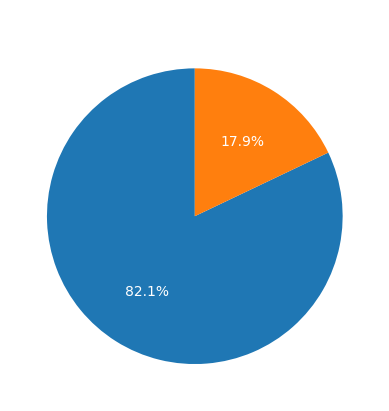
\includegraphics[scale=0.55]{./images/ill_extra.png}
        \end{figure}
      \end{column}
      \begin{column}{0.50\textwidth}
        \begin{figure}
          \centering
          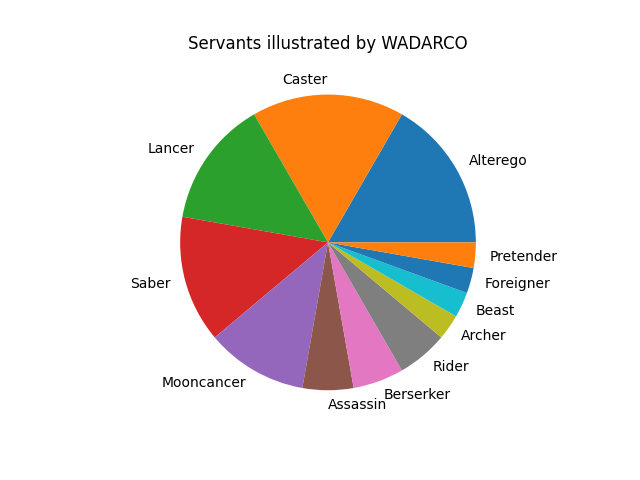
\includegraphics[scale=0.55]{./images/wadarco.png}
        \end{figure}
      \end{column}
    \end{columns}
  \end{frame}

  \begin{frame}{Conclusioni}
    \textbf{Grazie per l'attenzione.}
  \end{frame}

\end{darkframes}

\end{document}

